\section{Desarrollo}

\subsection*{Parte 1: Madurez}

En primer lugar, se determina la madurez del hormigón según el método de Plowman, para luego calcular el tiempo necesario para alcanzar la resistencia requerida mediante los métodos de Nurse-Saul, como los de Freiesleben, Hansen y Pedersen.

\subsubsection*{Método de Plowman}

Considerando una temperatura del terreno de 23.00 °C ($T_r$) y un valor de $T_D = 0.00$ °C, se calcula la madurez como:

\begin{equation}
    M = t_{eq} (T_r - T_D) \quad \text{donde} \quad t_{eq} = 13.27
\end{equation}

A partir de los datos entregados, se obtiene la siguiente tabla:

\begin{table}[H]
\centering
\renewcommand{\arraystretch}{1.15}
\caption{Cálculo de madurez del hormigón según método de Plowman}
\begin{tabular}{r r r r r r r }
\hline
\multicolumn{1}{c}{Edad [días]} & \multicolumn{1}{c}{Temperatura [°C]} & \multicolumn{1}{c}{Resistencia [MPa]} & \multicolumn{1}{c}{$\Delta t$ [días]} & \multicolumn{1}{c}{$T_{prom}$ [°C]} & \multicolumn{1}{c}{Madurez [°C·h]} & \multicolumn{1}{c}{Madurez [°C·día]} \\
\hline
0.00 & 29.00 & 0.00 & 0.00 & -- & 0.00 & 0.00\\
0.25 & 39.00 & 0.39 & 0.25 & 34.00 & 8.50 & 7.00 \\
0.50 & 49.00 & 0.88 & 0.25 & 44.00 & 19.50 & 14.00 \\
0.75 & 54.00 & 1.42 & 0.25 & 51.50 & 32.38 & 21.00 \\
1.00 & 59.00 & 2.01 & 0.25 & 56.50 & 46.50 & 28.00 \\
1.50 & 64.00 & 3.29 & 0.50 & 61.50 & 77.25 & 42.00  \\
2.00 & 59.00 & 4.47 & 0.50 & 61.50 & 108.00 & 56.00  \\
2.50 & 48.00 & 5.43 & 0.50 & 53.50 & 134.75 & 70.00  \\
3.00 & 44.00 & 6.31 & 0.50 & 46.00 & 157.75 & 84.00  \\
3.50 & 39.00 & 7.09 & 0.50 & 41.50 & 178.50 & 98.00  \\
4.00 & 34.00 & 7.77 & 0.50 & 36.50 & 196.75 & 112.00  \\
4.50 & 29.00 & 8.35 & 0.50 & 31.50 & 212.50 & 126.00  \\
5.00 & 26.00 & 8.87 & 0.50 & 27.50 & 226.25 & 140.00  \\
5.50 & 26.00 & 9.39 & 0.50 & 26.00 & 239.25 & 154.00  \\
6.00 & 23.00 & 9.85 & 0.50 & 24.50 & 251.50 & 168.00  \\
7.00 & 23.00 & 10.77 & 1.00 & 23.00 & 274.50 & 196.00  \\
8.00 & 23.00 & 11.69 & 1.00 & 23.00 & 297.50 & 224.00  \\
9.00 & 23.00 & 12.61 & 1.00 & 23.00 & 320.50 & 252.00  \\
10.00 & 23.00 & 13.53 & 1.00 & 23.00 & 343.50 & 280.00  \\
11.00 & 23.00 & 14.45 & 1.00 & 23.00 & 366.50 & 308.00  \\
14.00 & 23.00 & 17.21 & 3.00 & 23.00 & 435.50 & 392.00  \\
21.00 & 23.00 & 23.65 & 7.00 & 23.00 & 596.50 & 588.00  \\
28.00 & 23.00 & 30.09 & 7.00 & 23.00 & 757.50 & 784.00  \\
\hline
\end{tabular}
Fuente: Elaboración propia.
\end{table}

De esta manera, al interpolar la madurez obtenida, se obtiene un tiempo de 8.33 días, es decir, el tiempo necesario para que el hormigón en obra alcance una resistencia similar a la lograda en laboratorio a los 13.27 días.

Ahora es necesario determinar la madurez del hormigón al 85\% de $f_{cm}$. Considerando un hormigón G20 con una desviación estándar de 4.00 MPa, se obtiene:

\begin{equation}
    0.85 \cdot f_{cm} = f'_c + t \cdot s = (20.00 + 1.282 \cdot 4.00)\cdot 0.85 = 21.35\ \text{MPa}
\end{equation}

Luego se obtienen los factores $K_1$ y $K_2$ a partir de los valores a 3 y 28 días:

\begin{equation}
    6.31 = K_1 + K_2 \log(2016)
\end{equation}

\begin{equation}
    30.09 = K_1 + K_2 \log(18816)
\end{equation}

De esta forma, $K_1 = -74.70$ y $K_2 = 24.51$. Por lo tanto, la madurez requerida es:

\begin{equation}
    R(M) = K_1 + K_2 \log(M)
\end{equation}

\begin{equation}
    21.35 = -74.70 + 24.51 \log(M)
\end{equation}

\noindent Así, la madurez necesaria es de $M = 345.26\ °C\cdot día$.

\subsubsection*{Método de Nurse–Saul}

El método establece que el tiempo equivalente puede calcularse mediante la siguiente expresión:

\begin{equation}
    \Delta t_{eq} = \frac{T_i - T_d}{T_r - T_d} \Delta t_i
\end{equation}

De esta forma, se obtiene la siguiente tabla:

\begin{table}[H]
\centering
\renewcommand{\arraystretch}{1.15}
\caption{Cálculo del tiempo equivalente según el método de Nurse–Saul}
\begin{tabular}{r r r r r}
\hline
\multicolumn{1}{c}{Edad [días]} & \multicolumn{1}{c}{Temperatura [°C]} & \multicolumn{1}{c}{$t_{eq,i}$ obra [días]} & \multicolumn{1}{c}{$t_{eq,i}$ lab [días]} & \multicolumn{1}{c}{Madurez [°C·día]} \\
\hline
0.00 & 29.00 & 0.00 & 0.00 & 0.00 \\
0.25 & 39.00 & 0.42 & 0.39 & 7.00 \\
0.50 & 49.00 & 0.96 & 0.88 & 14.00 \\
0.75 & 54.00 & 1.54 & 1.42 & 21.00 \\
1.00 & 59.00 & 2.18 & 2.01 & 28.00 \\
1.50 & 64.00 & 3.58 & 3.29 & 42.00 \\
2.00 & 59.00 & 4.86 & 4.47 & 56.00 \\
2.50 & 48.00 & 5.90 & 5.43 & 70.00 \\
3.00 & 44.00 & 6.86 & 6.31 & 84.00 \\
3.50 & 39.00 & 7.71 & 7.09 & 98.00 \\
4.00 & 34.00 & 8.45 & 7.77 & 112.00 \\
4.50 & 29.00 & 9.08 & 8.35 & 126.00 \\
5.00 & 26.00 & 9.64 & 8.87 & 140.00 \\
5.50 & 26.00 & 10.21 & 9.39 & 154.00 \\
6.00 & 23.00 & 10.71 & 9.85 & 168.00 \\
7.00 & 23.00 & 11.71 & 10.77 & 196.00 \\
8.00 & 23.00 & 12.71 & 11.69 & 224.00 \\
9.00 & 23.00 & 13.71 & 12.61 & 252.00 \\
10.00 & 23.00 & 14.71 & 13.53 & 280.00 \\
11.00 & 23.00 & 15.71 & 14.45 & 308.00 \\
14.00 & 23.00 & 18.71 & 17.21 & 392.00 \\
21.00 & 23.00 & 25.71 & 23.65 & 588.00 \\
28.00 & 23.00 & 32.71 & 30.09 & 784.00 \\
\hline
\end{tabular}

Fuente: Elaboración propia.

\end{table}

Al interpolar la madurez obtenida, se determina un tiempo de 17.04 días en obra y 15.67 días en laboratorio para alcanzar la resistencia requerida de 21.35 MPa.


\subsection*{Método de Freiesleben Hansen y Pedersen}

El método establece que el tiempo equivalente puede calcularse mediante la siguiente expresión:

\begin{equation}
    t_{eq} = \sum e^{-Q \cdot \left(\frac{1}{T_a} - \frac{1}{T_s}\right)} \Delta t_i
\end{equation}

Donde $Q$ corresponde a la energía de activación. Para un cemento tipo I, $Q = 5000$, y por simplicidad se considera que para un cemento tipo II este valor no varía.  
A partir de estos parámetros, se obtiene la siguiente tabla:

\begin{table}[H]
\centering
\renewcommand{\arraystretch}{1.15}
\caption{Cálculo del tiempo equivalente según el método de Freiesleben Hansen y Pedersen}
\begin{tabular}{r r r r r r}
\hline
\multicolumn{1}{c}{Edad [días]} & \multicolumn{1}{c}{Temperatura [°C]} & \multicolumn{1}{c}{Madurez [°C·día]} & \multicolumn{1}{c}{$K_{prom}$ [K]} & \multicolumn{1}{c}{$t_{eq}$ obra [días]} & \multicolumn{1}{c}{$t_{eq}$ lab [días]} \\
\hline
0.00 & 29.00 & 0.00 & 273.15 & 0.00 & 0.00 \\
0.25 & 39.00 & 7.00 & 307.15 & 0.46 & 0.41 \\
0.50 & 49.00 & 14.00 & 317.15 & 1.22 & 1.09 \\
0.75 & 54.00 & 21.00 & 324.65 & 2.32 & 2.07 \\
1.00 & 59.00 & 28.00 & 329.65 & 3.71 & 3.32 \\
1.50 & 64.00 & 42.00 & 334.65 & 7.20 & 6.43 \\
2.00 & 59.00 & 56.00 & 334.65 & 10.69 & 9.54 \\
2.50 & 48.00 & 70.00 & 326.65 & 13.11 & 11.70 \\
3.00 & 44.00 & 84.00 & 319.15 & 14.80 & 13.21 \\
3.50 & 39.00 & 98.00 & 314.65 & 16.14 & 14.42 \\
4.00 & 34.00 & 112.00 & 309.65 & 17.19 & 15.35 \\
4.50 & 29.00 & 126.00 & 304.65 & 17.99 & 16.06 \\
5.00 & 26.00 & 140.00 & 300.65 & 18.63 & 16.64 \\
5.50 & 26.00 & 154.00 & 299.15 & 19.22 & 17.17 \\
6.00 & 23.00 & 168.00 & 297.65 & 19.77 & 17.65 \\
7.00 & 23.00 & 196.00 & 296.15 & 20.77 & 18.55 \\
8.00 & 23.00 & 224.00 & 296.15 & 21.77 & 19.44 \\
9.00 & 23.00 & 252.00 & 296.15 & 22.77 & 20.33 \\
10.00 & 23.00 & 280.00 & 296.15 & 23.77 & 21.22 \\
11.00 & 23.00 & 308.00 & 296.15 & 24.77 & 22.12 \\
14.00 & 23.00 & 392.00 & 296.15 & 27.77 & 24.80 \\
21.00 & 23.00 & 588.00 & 296.15 & 34.77 & 31.05 \\
28.00 & 23.00 & 784.00 & 296.15 & 41.77 & 37.30 \\
\hline
\end{tabular}

Fuente: Elaboración propia.

\end{table}

Al interpolar la madurez obtenida, se obtiene un tiempo de 26.10 días en obra y 23.31 días en laboratorio para alcanzar la resistencia requerida de 21.35 MPa.

Las diferencias entre ambos métodos radican en que el modelo de Nurse–Saul es más simple y lineal, ya que no considera los efectos de la reacción química. En cambio, el modelo de Freiesleben Hansen y Pedersen incorpora la energía de activación y la variación de temperatura en una formulación exponencial, lo que lo hace más preciso para predecir la resistencia del hormigón en función del tiempo y la temperatura. 

Cabe destacar que la energía de activación en este último método cumple un rol fundamental: a mayores valores de $Q$, el tiempo equivalente aumenta, lo que implica una reacción más lenta del hormigón.


\subsection*{Parte 2: Presión de Moldajes}

Se tienen los siguientes datos de entrada:

\begin{table}[H]
\centering
\renewcommand{\arraystretch}{1.20}
\caption{Datos de entrada para el cálculo de presión de moldajes}
\begin{tabular}{c c c c c c}
\hline
\begin{tabular}{@{}c@{}}Tipo\\ de Cemento\end{tabular} &
\begin{tabular}{@{}c@{}}Cono de\\ Asentamiento (mm)\end{tabular} &
\begin{tabular}{@{}c@{}}Densidad\\ (kg/m\textsuperscript{3})\end{tabular} &
\begin{tabular}{@{}c@{}}Altura de\\ Colocación (m)\end{tabular} &
\begin{tabular}{@{}c@{}}Temperatura\\ ($^\circ$C)\end{tabular} &
\begin{tabular}{@{}c@{}}Presión\\ Lateral (kPa)\end{tabular} \\
\hline
II & 148.00 & 2376.00 & 6.10 & 16.40 & 89.00 \\
\hline
\end{tabular}

Fuente: Elaboración propia.

\end{table}

Los valores se ingresaron en la calculadora de presión de moldajes de \href{https://apps.peri.com/SLR/index.php?lang=en&norm=aci}{PERI}. La configuración utilizada se muestra a continuación:

\begin{figure}[H]
    \centering
    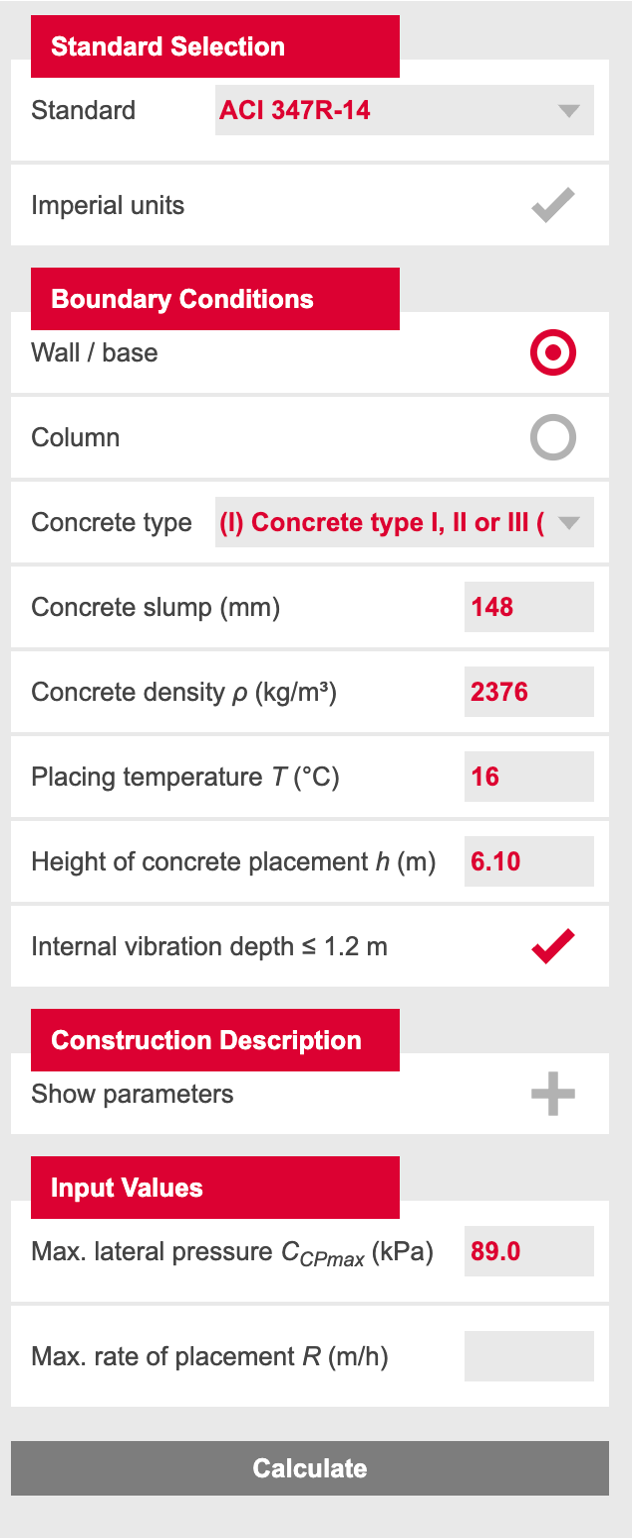
\includegraphics[width=0.40\linewidth]{datos_entrada.png}
    \caption{Datos ingresados en la calculadora de PERI}
    
    Fuente: Elaboración propia.
    
\end{figure}

El resultado obtenido es el siguiente:

\begin{figure}[H]
    \centering
    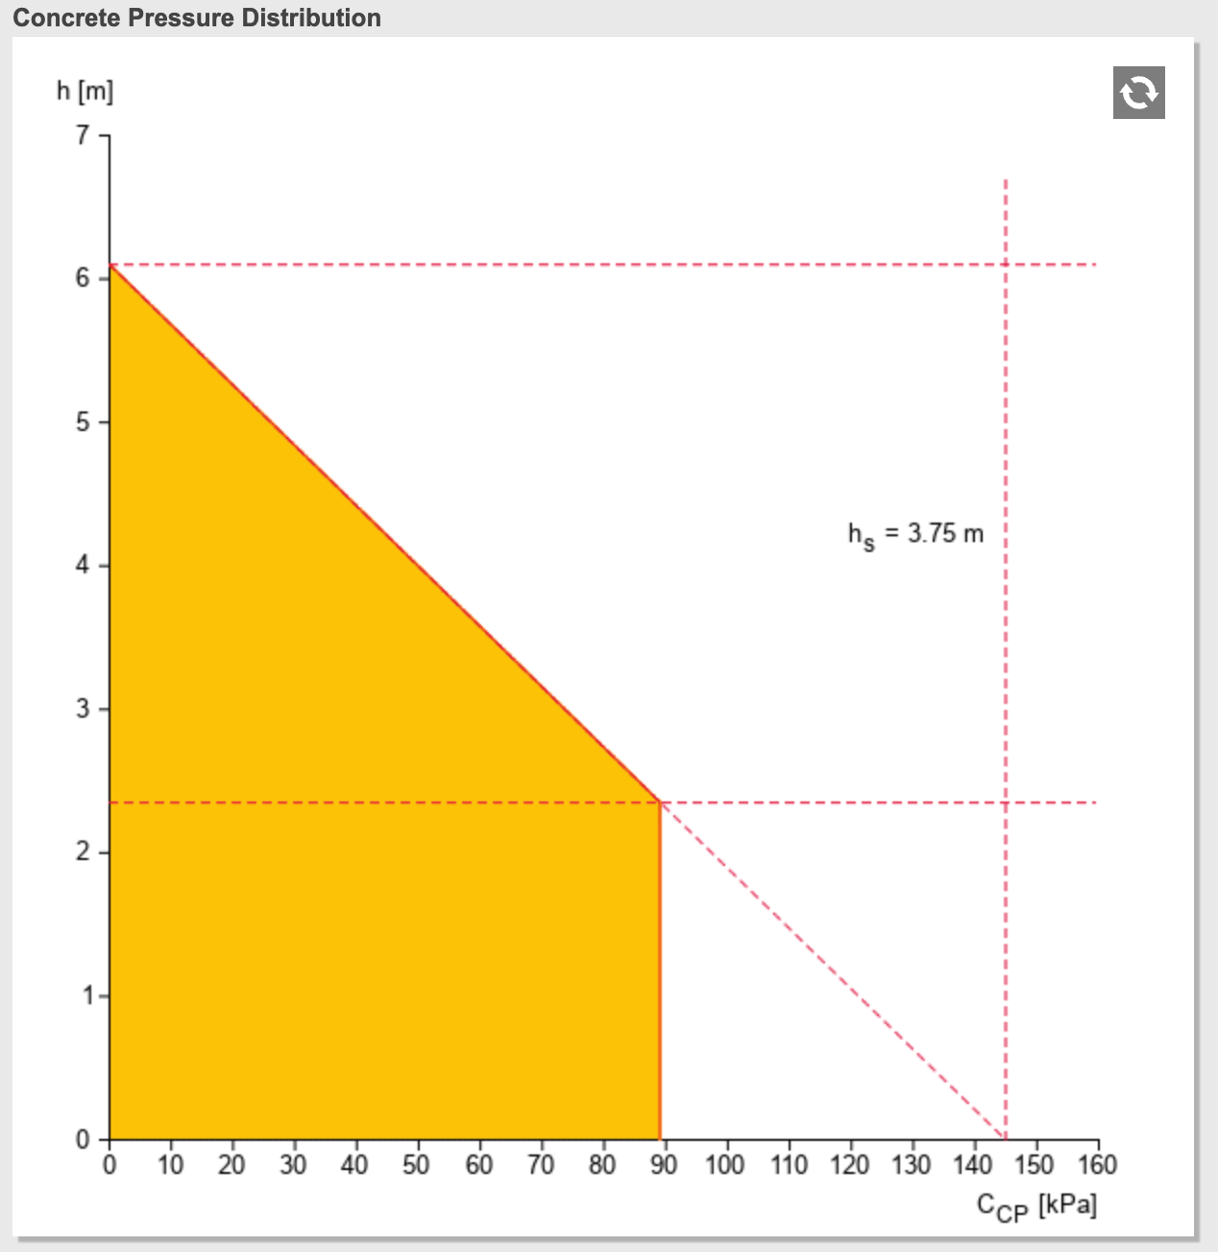
\includegraphics[width=0.50\linewidth]{resultado.png}
    \caption{Resultado de la calculadora de PERI}
    
    Fuente: Elaboración propia.
    
\end{figure}

No se genera un límite de hormigonado; por lo tanto, se puede realizar la solicitud de \(10~\mathrm{m/h}\) sin inconvenientes.

Ahora bien, si la presión máxima admisible es el \(80\,\%\) de la indicada, es decir, \(71.20~\mathrm{kPa}\), para mantener el rendimiento de \(10~\mathrm{m/h}\) se propone disminuir la densidad del hormigón a \(2150.00~\mathrm{kg/m^3}\). Con este ajuste, el resultado es:

\begin{figure}[H]
    \centering
    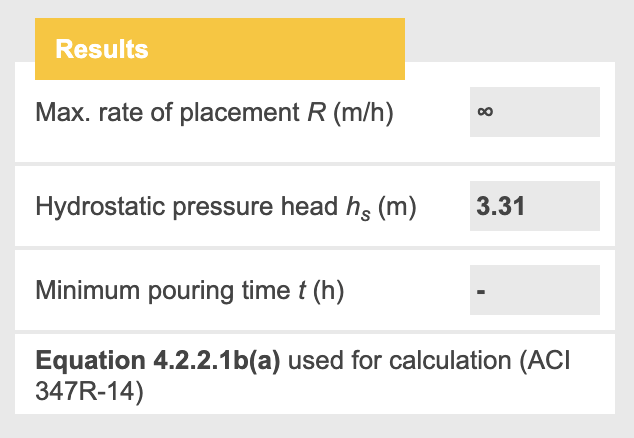
\includegraphics[width=0.50\linewidth]{max_rate.png}
    \caption{Resultado de la calculadora de PERI con densidad reducida}
Fuente: Elaboración propia.

\end{figure}

La distribución de presiones resultante es la siguiente:

\begin{figure}[H]
    \centering
    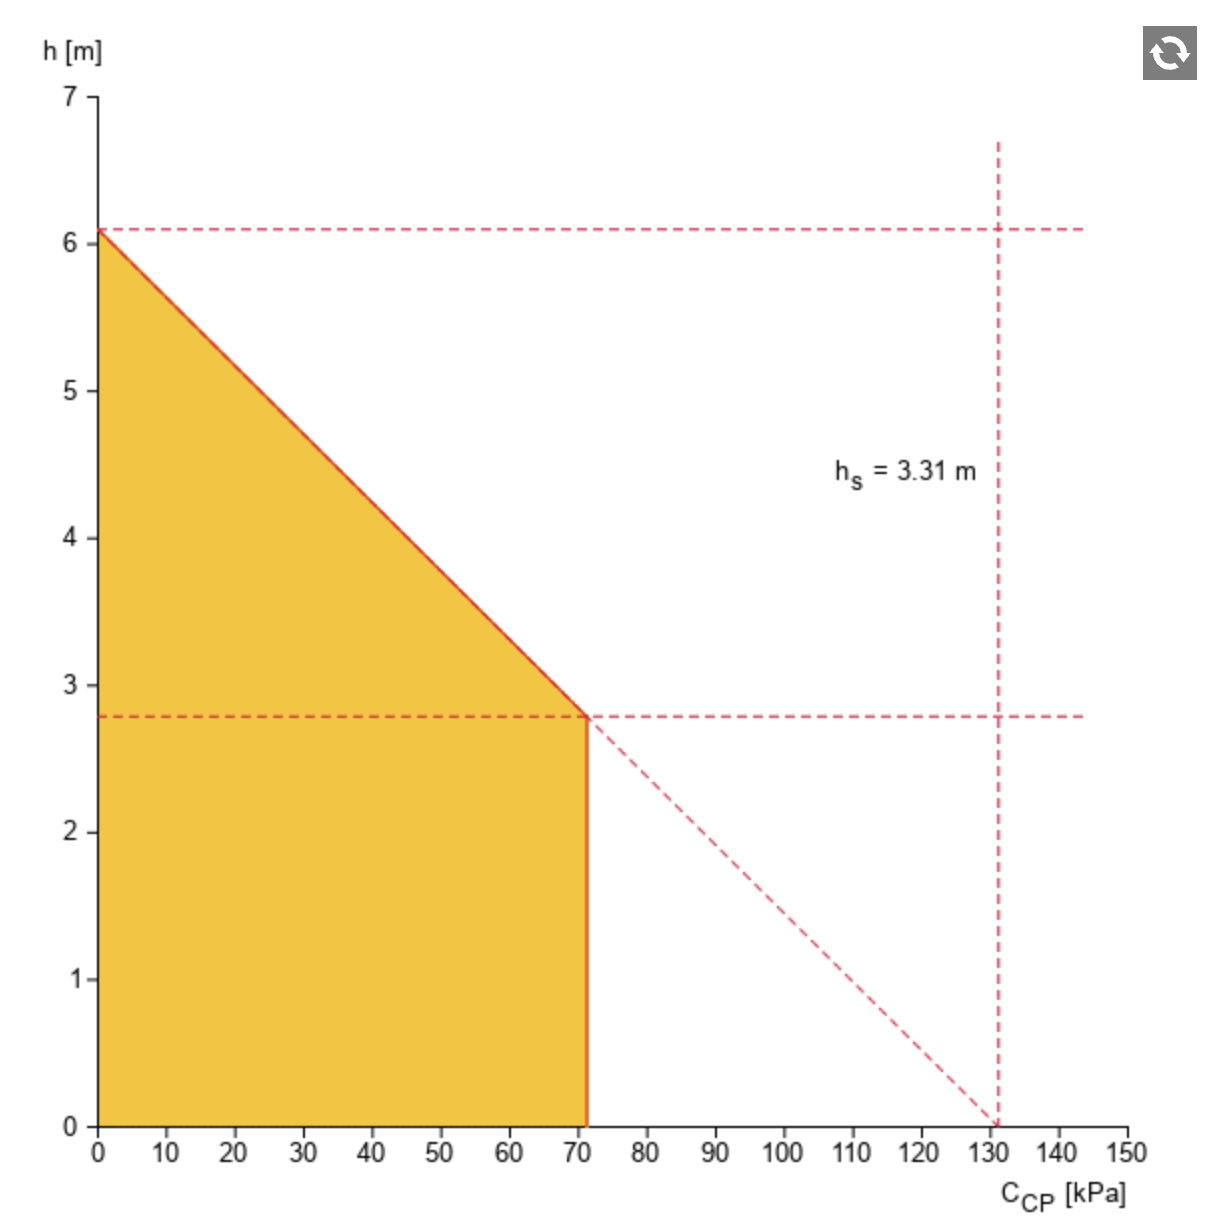
\includegraphics[width=0.50\linewidth]{presiones_2.png}
    \caption{Distribución de presión con densidad reducida}
Fuente: Elaboración propia.

\end{figure}

Para lograr este objetivo, puede emplearse un hormigón con agregados livianos a fin de reducir la densidad fresca y, en consecuencia, la presión lateral sobre los moldajes.

\subsection*{Parte 3: Método de Bolomey y Venuat}

En esta parte se determinó el tiempo mínimo de desmolde de una columna con el objetivo de optimizar el presupuesto de la obra. Se compararon los tiempos de desmolde obtenidos al emplear un hormigón tradicional y uno de alta resistencia.  

Para el desarrollo de esta sección se aplicaron los métodos de Bolomey y Venuat, los cuales permiten estimar la resistencia del hormigón en función de su dosificación y del tiempo de curado.

A continuación, se presentan los datos experimentales, los cálculos efectuados para ambos tipos de hormigón y los resultados obtenidos.

\begin{table}[H]
\centering
\renewcommand{\arraystretch}{1.15}
\caption{Datos experimentales – Grupo 5}
\small
\begin{tabular}{lccc}
\hline
\textbf{Parámetro} & \textbf{Unidad} & \textbf{Cem. corriente} & \textbf{Cem. alta resistencia} \\ \hline
Agua utilizada & kg/m$^3$ & 166.32 & 153.68 \\
Cemento mezcla 1 (Z1 / V1) & kg/m$^3$ & 432.23 & 324.68 \\
Cemento mezcla 2 (Z2 / V2) & kg/m$^3$ & 312.42 & 381.65 \\
Resistencia 14 días mezcla 1 & MPa & 20.45 & 24.24 \\
Resistencia 14 días mezcla 2 & MPa & 15.47 & 33.20 \\
Resistencia 28 días mezcla 1 & MPa & 27.27 & 29.55 \\
Resistencia 28 días mezcla 2 & MPa & 22.42 & 43.11 \\
Agua para columnas & kg/m$^3$ & 141.00 & 141.00 \\ \hline
\end{tabular}
\begin{center}
Fuente: Elaboración propia.
\end{center}
\end{table}

\subsubsection*{Resistencia a la compresión}

En primer lugar, se determinó la resistencia requerida a partir de la resistencia especificada, utilizando la siguiente expresión:
\[
f_{cm} = f'_c + t \cdot s
\]
donde $f'_c$ es la resistencia especificada, $t$ es el factor de seguridad y $s$ corresponde a la desviación estándar del hormigón.

\begin{table}[H]
\centering
\renewcommand{\arraystretch}{1.15}
\caption{Resistencia requerida para el desmolde}
\begin{tabular}{lcc}
\hline
\textbf{Parámetro} & \textbf{Símbolo} & \textbf{Valor [MPa]} \\ \hline
Desviación estándar & $s$ & 3.42 \\
Factor de seguridad & $t$ & 2.11 \\
Resistencia especificada & $f'_c$ & 28.86 \\
Resistencia requerida & $f_{cm}$ & 36.08 \\
Porcentaje requerido & -- & 90.00 \\
Resistencia mínima para desmolde & $f_{req}$ & 32.47 \\ \hline
\end{tabular}
\begin{center}
Fuente: Elaboración propia.
\end{center}
\end{table}

\subsubsection*{Dosis mínima de cemento}

En segundo lugar, se aplicó el método de Bolomey para determinar la dosis mínima de cemento necesaria para alcanzar la resistencia requerida.  
El método se basa en la siguiente relación empírica:

\[
R = a\left(\frac{c}{w} - b\right)
\]

donde $R$ es la resistencia del hormigón, $c/w$ es la relación cemento/agua, y $a$, $b$ son parámetros característicos del material, determinados experimentalmente a 14 y 28 días.  

Los sistemas de ecuaciones resueltos son los siguientes:

Para el cemento corriente:
\[
\begin{cases}
20.45 = a_{14}(3.07 - b_{14}) \\
15.47 = a_{14}(2.22 - b_{14})
\end{cases}
\quad
\begin{cases}
27.27 = a_{28}(3.07 - b_{28}) \\
22.42 = a_{28}(2.22 - b_{28})
\end{cases}
\]

Para el cemento de alta resistencia:
\[
\begin{cases}
24.24 = a_{14}(2.31 - b_{14}) \\
33.20 = a_{14}(2.71 - b_{14})
\end{cases}
\quad
\begin{cases}
29.55 = a_{28}(2.31 - b_{28}) \\
43.11 = a_{28}(2.71 - b_{28})
\end{cases}
\]

\begin{table}[H]
\centering
\renewcommand{\arraystretch}{1.15}
\caption{Parámetros obtenidos por el método de Bolomey para cada tipo de cemento}
\small
\begin{tabular}{lcc}
\hline
\textbf{Parámetro} & \textbf{Cem. corriente} & \textbf{Cem. alta resistencia} \\ \hline
$c/w$ – Mezcla 1 (Z1 / V1) & 3.07 & 2.31 \\
$c/w$ – Mezcla 2 (Z2 / V2) & 2.22 & 2.71 \\
$a_{14}$ & 5.85 & 22.15 \\
$b_{14}$ & -0.42 & 1.21 \\
$a_{28}$ & 5.70 & 33.51 \\
$b_{28}$ & -1.72 & 1.42 \\
$c/w$ (promedio) & 4.62 & 2.50 \\
$c$ & 650.12~[kg/m$^3$] & 352.10~[kg/m$^3$] \\ \hline
\end{tabular}
\begin{center}
Fuente: Elaboración propia.
\end{center}
\end{table}

\subsubsection*{Tiempo de desmolde}

En esta sección se aplicó el método de Venuat para determinar el tiempo mínimo de desmolde en ambos tipos de cemento.  
El método se basa en la relación entre la resistencia del hormigón y el tiempo de curado, expresada de forma logarítmica mediante la siguiente ecuación:

\[
R = K_1 + K_2 \cdot \log_{10}(t)
\]

Los sistemas resueltos fueron los siguientes:

\textbf{Cemento corriente:}
\[
\begin{cases}
29.51 = K_1 + K_2 \cdot \log_{10}(14) \\
36.08 = K_1 + K_2 \cdot \log_{10}(28)
\end{cases}
\]

\textbf{Cemento de alta resistencia:}
\[
\begin{cases}
28.55 = K_1 + K_2 \cdot \log_{10}(14) \\
36.08 = K_1 + K_2 \cdot \log_{10}(28)
\end{cases}
\]

Posteriormente, se despejó el tiempo necesario para alcanzar la resistencia mínima requerida para el desmolde, utilizando la misma ecuación de Venuat.  
Los valores obtenidos se presentan a continuación:

\begin{table}[H]
\centering
\renewcommand{\arraystretch}{1.15}
\caption{Constantes obtenidas mediante el método de Venuat}
\small
\begin{tabular}{lcccc}
\hline
\textbf{Tipo de cemento} & \textbf{$R_{14}$ [MPa]} & \textbf{$K_1$} & \textbf{$K_2$} & \textbf{$t_{desmolde}$ [días]} \\ \hline
Cemento corriente & 29.51 & 4.48 & 21.84 & 19.14 \\
Cemento alta resistencia & 28.55 & -0.13 & 25.02 & 20.09 \\ \hline
\end{tabular}
\begin{center}
Fuente: Elaboración propia.
\end{center}
\end{table}

\subsubsection*{Comparación de costos del proyecto}

A partir de los tiempos de desmolde obtenidos y los costos asociados a cada variable, se elaboró el siguiente análisis comparativo:

\begin{table}[H]
\centering
\renewcommand{\arraystretch}{1.10}
\caption{Análisis de costos por tipo de cemento}
\small
\begin{tabular}{lcccc}
\hline
\textbf{Concepto} & \textbf{Unidad} & \textbf{Cem. corriente} & \textbf{Cem. alta resistencia} \\ \hline
Costo del cemento & \$/kg & 100.00 & 140.00 \\
Costo de moldajes & \$/día & 400.00 & 400.00 \\
Consumo de cemento & kg/m$^3$ & 650.12 & 352.10 \\
Duración del moldaje & días & 19.14 & 20.09 \\
Costo total por 1 m$^3$ & \$ & 72,668.00 & 57,329.00 \\ \hline
\end{tabular}
\begin{center}
Fuente: Elaboración propia.
\end{center}
\end{table}

A partir de los resultados obtenidos mediante los métodos de Bolomey y Venuat, se observa que el uso de cemento de alta resistencia inicial presenta una mejor relación entre consumo de material, resistencia alcanzada y costo total por metro cúbico de hormigón.

Aunque el costo unitario del cemento de alta resistencia es mayor, la menor dosificación requerida compensa la diferencia.  

El tiempo estimado de desmolde es similar: 19.14 días para el cemento corriente y 20.09 días para el cemento de alta resistencia, diferencia que no afecta significativamente el proceso constructivo.

Finalmente, al integrar ambos factores en el análisis económico, el costo total del elemento resulta menor para el cemento de alta resistencia (57,329 \$ por m$^3$), en comparación con el cemento corriente (72,668 \$ por m$^3$).  

Por lo tanto, la alternativa más eficiente desde el punto de vista técnico y económico es el uso de cemento de alta resistencia, ya que permite alcanzar la resistencia requerida con menor consumo de material y menor costo total, manteniendo un desempeño estructural equivalente.

\newpage
\subsection*{Discusión}

\subsubsection*{Pregunta 1} 
La velocidad de colocación influye directamente en la distribución de la presión lateral del hormigón fresco.  
Cuando la colocación es rápida, el hormigón no alcanza a fraguar en las capas inferiores, generando una pseudo presión hidrostática sobre los moldajes. En cambio, una colocación lenta permite que las primeras capas comiencen a endurecerse, reduciendo los esfuerzos laterales.  

El bombeo continuo o el vertido en capas controladas modifican esta distribución, mientras que el vibrado interno es un factor adicional que puede aumentar la presión lateral al reducir temporalmente la viscosidad del material.


\subsubsection*{Pregunta 2} 
A mayor temperatura, se acelera el fraguado y la pérdida de trabajabilidad, reduciendo el tiempo durante el cual el hormigón ejerce presión máxima sobre los moldajes. En cambio, a bajas temperaturas el proceso de hidratación se ralentiza, aumentando el tiempo en que el material mantiene un comportamiento casi hidrostático.  

Las temperaturas extremas pueden alterar la microestructura del cemento: en climas cálidos aumenta la evaporación superficial y la retracción plástica, mientras que en climas fríos puede producirse congelamiento del agua y retraso del endurecimiento.  
Por lo tanto, los factores climáticos deben considerarse al definir las tasas de colocación, los tiempos de fraguado y los plazos de descimbre.


\subsubsection*{Pregunta 3} 

Un cálculo conservador de la presión sobre los moldajes se obtiene considerando la columna de hormigón, es decir:

\begin{equation}
    p = \gamma \cdot g \cdot h
\end{equation}

donde $h$ corresponde a la altura de colocación. Por lo tanto, la presión tiene una relación directamente proporcional con la altura del elemento.  

En la práctica —y como se observó en el desarrollo del taller— la presión máxima real es menor que la calculada teóricamente, debido al fraguado progresivo del hormigón y a la interacción interna de la pasta de cemento.  

Este factor adquiere gran relevancia al hormigonar elementos de gran altura o con difícil acceso, ya que complica la disposición de puntales y el control de la velocidad de colocación, lo que puede generar presiones superiores a las previstas.  
Asimismo, la consideración de este factor es crítica en construcciones con moldajes deslizantes, donde la velocidad de ascenso del molde debe controlarse cuidadosamente para evitar presiones excesivas que comprometan la estabilidad estructural.


\subsubsection*{Pregunta 4} 

Las principales ventajas del método de madurez radican en que permite estimar la resistencia del hormigón en obra a partir de datos obtenidos en laboratorio, facilitando un control continuo de calidad sin afectar el proceso constructivo.  

Sin embargo, presenta limitaciones frente a elementos masivos, en los que las variaciones de temperatura interna pueden ser significativas y generar errores en la estimación de la resistencia. Además, el método requiere un monitoreo constante de la temperatura, lo que implica la instalación de sensores en ubicaciones clave, personal especializado y costos adicionales.  

Otros factores, como la geometría del elemento, también influyen: los elementos delgados disipan el calor más rápidamente que los de gran volumen (por ejemplo, fundaciones aisladas).  
Asimismo, las condiciones de curado y el clima ambiente afectan la ganancia de resistencia, pudiendo acelerar o inhibir la reacción de hidratación del cemento.  

En consecuencia, el método de madurez tiende a ser más preciso en elementos delgados y convencionales (como losas, vigas o muros), mientras que en estructuras masivas o con curado no controlado puede presentar limitaciones significativas.

\subsubsection*{Pregunta 5} 

El tipo de cemento afecta significativamente la estimación de madurez, especialmente en el método de Freiesleben Hansen y Pedersen, dado que la energía de activación ($Q$) varía entre los distintos tipos de cemento.  
Cementos con mayor contenido de clínker o con aditivos especiales presentan diferentes tasas de reacción, lo que modifica la velocidad de ganancia de resistencia.  

En el método de Nurse–Saul, el tipo de cemento influye de manera indirecta a través de la temperatura alcanzada durante la hidratación, pero no interviene explícitamente en la ecuación.

Por otro lado, si la presión ejercida por el hormigón se calcula únicamente mediante la estimación hidrostática (columna de hormigón), el tipo de cemento tiene poca incidencia, ya que no se esperan variaciones significativas en la densidad del material.  
Sin embargo, si se consideran factores como la velocidad de colocación, el fraguado y la pérdida de trabajabilidad, el tipo de cemento puede afectar indirectamente la presión ejercida: cementos de fraguado rápido tienden a reducir la presión máxima al acelerar el endurecimiento del hormigón.

Algunos materiales cementantes suplementarios (SCM) también modifican este comportamiento. Por ejemplo, la \textit{fly ash} (ceniza volante) retrasa el fraguado, ya que sus partículas reaccionan lentamente con el hidróxido de calcio, disminuyendo el calor de hidratación y prolongando el tiempo de presión sobre los moldajes.  
De forma similar, la escoria de alto horno reacciona con el hidróxido de calcio, retardando el fraguado y manteniendo la presión lateral por más tiempo.  
En contraste, la sílice fume (\textit{silica fume}) es altamente reactiva, incrementando notablemente el calor de hidratación en edades tempranas, lo que acelera la ganancia de resistencia y reduce el tiempo durante el cual el hormigón ejerce presión sobre los moldajes.


\subsubsection*{Pregunta 6} 

El método de Bolomey relaciona la resistencia a compresión con la dosificación y la razón agua/cemento (w/c), mientras que el método de madurez se basa en la evolución térmica del hormigón para estimar su resistencia real en obra.  

Bolomey resulta útil para estimaciones iniciales o en contextos donde no se dispone de registros térmicos, pues permite definir la dosificación óptima de materiales bajo condiciones de curado estándar.  
Por su parte, el método de madurez permite un monitoreo en tiempo real del desarrollo resistente, considerando directamente las variaciones de temperatura y las condiciones ambientales del proyecto.

En síntesis, el método de Bolomey asume condiciones de curado estables, mientras que el de madurez las incorpora explícitamente.  
Por ello, en proyectos que requieren mayor precisión operativa y control estructural, el método de madurez es preferible. En cambio, para el control de planta y diseño de mezclas, el método de Bolomey resulta más práctico y eficiente.


\subsubsection*{Pregunta 7} 

Las constantes \(a\) y \(b\) del modelo de Bolomey representan la sensibilidad del hormigón frente a variaciones en la dosificación y en la calidad de los materiales.  
Cambios en el tipo de cemento, la granulometría o la naturaleza de los agregados modifican la relación efectiva \(c/w\) y, por tanto, la pendiente (\(a\)) y el intercepto (\(b\)) de la ecuación.

Ante un cambio de materiales, es necesario realizar ensayos de resistencia a distintas relaciones \(c/w\) para recalibrar los parámetros \(a\) y \(b\).  
Esto permite mantener la exactitud del modelo en la predicción de resistencias, garantizando la reproducibilidad del comportamiento mecánico del hormigón.


\subsubsection*{Pregunta 8} 

Según la relación de Bolomey, la resistencia a compresión es directamente proporcional a \((c/w - b)\).  
Si se reduce la cantidad de cemento en un 10\,\% manteniendo constante la cantidad de agua, la relación \(c/w\) disminuirá en el mismo porcentaje, reduciendo proporcionalmente la resistencia esperada.  

Esta variación implica una menor resistencia inicial, cuya magnitud dependerá de los valores de \(b\) y del tipo de cemento empleado. En consecuencia, la reducción del contenido de cemento debe evaluarse cuidadosamente, ya que puede afectar tanto la resistencia mecánica como la durabilidad del elemento estructural.

\subsubsection*{Pregunta 9} 

Aplicando el método de Venuat, se obtiene el siguiente sistema de ecuaciones:

\begin{equation}
    17.21 = K_1 + K_2 \cdot \log_{10}(14)
\end{equation}

\begin{equation}
    30.09 = K_1 + K_2 \cdot \log_{10}(28)
\end{equation}

Resolviendo el sistema, se obtiene que \( K_1 = -31.83 \) y \( K_2 = 42.78 \).  
Luego, para determinar el tiempo necesario para alcanzar la resistencia requerida, se utiliza nuevamente la ecuación de Venuat:

\begin{equation}
    21.35 = -31.83 + 42.78 \cdot \log_{10}(t)
\end{equation}

Despejando, se obtiene un tiempo de 17.50 días para alcanzar la resistencia de \(21.35~\mathrm{MPa}\).


\subsubsection*{Pregunta 10} 

\begin{table}[H]
\centering
\renewcommand{\arraystretch}{1.20}
\caption{Comparación de resistencias originales y con +5\% de variación}
\small
\begin{tabular}{lcccccc}
\hline
\multirow{2}{*}{\textbf{Tipo de cemento}} & \multirow{2}{*}{\textbf{Mezcla}} & \multicolumn{2}{c}{\textbf{14 días [MPa]}} & \multicolumn{2}{c}{\textbf{28 días [MPa]}} \\
\cline{3-6}
 & & Original & +5\% & Original & +5\% \\
\hline
Cemento corriente & Z1 & 20.45 & 21.47 & 27.27 & 28.63 \\
Cemento corriente & Z2 & 15.47 & 16.24 & 22.42 & 23.54 \\
\hline
Cemento alta resistencia & V1 & 24.24 & 25.45 & 29.55 & 31.03 \\
Cemento alta resistencia & V2 & 33.20 & 34.86 & 43.11 & 45.27 \\
\hline
\end{tabular}
\begin{center}
Fuente: Elaboración propia.
\end{center}
\end{table}

Si las resistencias presentaran una variación de $\pm5\%$, los resultados se verían directamente afectados.  
Para ambos tipos de cemento, las resistencias se desplazarían respecto a los valores reales, provocando tiempos de descimbre inadecuados.  

Un aumento del 5\,\% podría generar una sobreestimación de resistencia, llevando a un desmolde prematuro, mientras que una disminución del 5\,\% prolongaría innecesariamente el tiempo de moldaje, incrementando los costos y afectando la programación de obra.

Estas variaciones pueden mitigarse mediante un control de calidad riguroso, monitoreo de temperatura \textit{in situ} y protocolos de verificación previos al desmolde, asegurando que las condiciones reales coincidan con las supuestas en el cálculo.

\begin{table}[H]
\centering
\renewcommand{\arraystretch}{1.20}
\caption{Tiempos de desmolde con un +5\% de variación en resistencias}
\small
\begin{tabular}{lccc}
\hline
\textbf{Tipo de cemento} & \textbf{$K_1$} & \textbf{$K_2$} & \textbf{Tiempo de desmolde [días]} \\ 
\hline
Cemento corriente & 23.42 & 8.75 & 10.84 \\ 
Cemento alta resistencia & 0.73 & 20.28 & 18.59 \\ 
\hline
\end{tabular}
\begin{center}
Fuente: Elaboración propia.
\end{center}
\end{table}

En consecuencia, las variaciones en los valores de resistencia afectan de forma directa los parámetros $K_1$ y $K_2$ del modelo de Venuat, alterando los tiempos estimados de desmolde.  
Esto resalta la importancia de realizar ensayos de control y verificación de resistencia antes del retiro de los moldajes, a fin de garantizar tanto la seguridad estructural como la eficiencia económica del proceso constructivo.
